\section{$\delta\! f$ Models}
    \BA{Introduction.}

    Take from here the the assumptions of:
    \begin{itemize}
        \item  Leading-order locality of $(\bfC_{ss'})_{ss'}$,
        \begin{equation}
            \bfC_{ss'}  \sim  \bfC_{ss'}^{(0)}.
        \end{equation}
        \item  Quasineutrality,
        \begin{align}
            \overline{\rho}_{\rmC}  \ll \overline{n}_{s}\max_{s}\{\rmq_{s}\},  &&
            \overline{\bfj}         \ll  \overline{n}_{s}\max_{s}\{\rmq_{s}\}\overline{\bfv}.
        \end{align}
    \end{itemize}

    \line

    \begin{definition}[$\delta\! f$ models]
        ``$\delta\! f$ models'' write the distribution functions $(f_{s})_{s}$ for each $s$ in the form
        \begin{equation}
            f_{s}(\bfx, \bfv; t)  =  f_{s}^{(0)}[(\rho_{s})_{s}|_{\bfx; t}, \bfp|_{\bfx; t}, E|_{\bfx; t}](\bfx, \bfv; t) + \delta\! f_{s}(\bfx, \bfv; t),
        \end{equation}
        where $\left(f_{s}^{(0)}\right)_{s}$ are those thermalized distributions solving the local thermal equilibrium condition for each $s$ (\ref{eqn:local leading-order Boltzmann equation}),
        \begin{multline}\label{eqn:thermal equilibrium identity}
            \frac{\rmq_{s}}{\rmm_{s}}\nabla_{\bfv}\cdot\left[f_{s}^{(0)}(\bfE + \bfv\wedge\bfB) - \sum_{s'}\rmq_{s'}\bfC_{ss'}^{(0)}\left[f_{s}^{(0)}, f_{s'}^{(0)}\right]\right]  \\
            =  \frac{\rho_{\rmC}}{\rho_{\rmM}}\nabla_{\bfv}\cdot\left[f_{s}^{(0)}\left(\bfE + \frac{1}{\rho_{\rmC}}\bfj^{(0)}\wedge\bfB\right) - \nabla_{\bfv}\left[f_{s}^{(0)}\left(\frac{1}{\rho_{\rmC}}\bfj^{(0)} - \bfu\right)\cdot\left(\bfE + \bfu\wedge\bfB\right)\right]\right],
        \end{multline}
        where $\bfj^{(0)}$ denotes the \emph{thermalized} current density,
        \begin{equation}
            \bfj^{(0)}  :=  \sum_{s}\int_{\bfv}f_{s}^{(0)}q_{s}\bfv,
        \end{equation}
        with moments:
        \begin{align}
            \forall s,          &\int_{\bfv}f_{s}^{(0)}\rmm_{s}                         &  &=  &          &\int_{\bfv}f_{s}\rmm_{s}                         &  &=  &  \rho_{s}  \label{eqn:background mass moment}  \\
                        \sum_{s}&\int_{\bfv}f_{s}^{(0)}\rmm_{s}\bfv                     &  &=  &  \sum_{s}&\int_{\bfv}f_{s}\rmm_{s}\bfv                     &  &=  &  \bfp  \\
                        \sum_{s}&\int_{\bfv}f_{s}^{(0)}\frac{1}{2}\rmm_{s}\|\bfv\|^{2}  &  &=  &  \sum_{s}&\int_{\bfv}f_{s}\frac{1}{2}\rmm_{s}\|\bfv\|^{2}  &  &=  &  E  \label{eqn:background energy moment}
        \end{align}
        Substituting these $f_{s}  \mapsto  f_{s}^{(0)} + \delta\! f_{s}$ into the Boltzmann equations (\ref{eqn:Boltzmann equation}) one can derive a:
        \begin{itemize}
            \item  Fluid (MHD) model in $(\rho_{s})_{s}$, $\bfp$, $E$, by taking moments, similar to what was done under the classical \emph{exact} thermalization assumption $f_{s}  =  f_{s}^{(0)}$ in Subsection \ref{cha:fluid models}.
            \item  Kinetic model in $(\delta\! f_{s})_{s}$, retrieved directly from the Boltzmann equations after substitution of the relevant time derivatives for the moments $(\rho_{s})_{s}$, $\bfp$, $E$ from the fluid model.
        \end{itemize}
    \end{definition}

    The thermal equilibrium identities (\ref{eqn:thermal equilibrium identity}) derive from the leading-order Boltzmann equation (\ref{eqn:local leading-order Boltzmann equation}),
    \begin{equation}
        \frac{\rmq_{s}}{\rmm_{s}}\nabla_{\bfv}\cdot\left[f_{s}^{(0)}(\bfE + \bfv\wedge\bfB) - \sum_{s'}\rmq_{s'}\bfC_{ss'}^{(0)}\left[f_{s}^{(0)}, f_{s'}^{(0)}\right]\right]  \sim  0,
    \end{equation}
    with the addition of forcing/heating-like terms on the right hand side (RHS), uniform in $s$, that are comparitively negligible due to quasineutrality, such that the relevant moments are 0 and the identities necessarily admit the $(S + 4)$-dimensional manifold of solutions.

    $\delta\! f$ models offer a way to recover an approachable fluid model from the Boltzmann equations \emph{without} the unreliable exact thermalization assumption $f_{s}  =  f_{s}^{(0)}$ or other techniques, at the expense of the introduction of the $(\delta\! f_{s})_{s}$ ``corrections'' which must also be modeled.

    \line

    \begin{lemma}[Moments on $(\delta\! f_{s})_{s}$]
        \begin{align}
            \forall s,          \int_{\bfv}\delta\! f_{s}\rmm_{s}                          =  0,  &&
                        \sum_{s}\int_{\bfv}\delta\! f_{s}\rmm_{s}\bfv                      =  \bfzero,  &&
                        \sum_{s}\int_{\bfv}\delta\! f_{s}\frac{1}{2}\rmm_{s}\|\bfv\|^{2}   =  0.
        \end{align}
    \end{lemma}
    \begin{proof}
        These are immediate from the moments (\ref{eqn:background mass moment}--\ref{eqn:background energy moment}) with $f_{s}  =  f_{s}^{(0)} + \delta\! f_{s}$.
    \end{proof}

    This condition is crucial for deriving the fluid model from the Boltzmann equations, as the time derivative in $(\delta\! f_{s})_{s}$ necessarily vanish after taking the relevant moments.

    \line
    
    Consider again the model from Section \ref{cha:fluid models} with:
    \begin{itemize}
        \item  Two phases: A mass-dominant positive ion phase, and negative electron phase.
        \item  Isotropic collisions, such that the moment identities (\ref{eqn:isotropic 2nd moment}--\ref{eqn:isotropic 3rd moment}) hold.
    \end{itemize}

    Substituting $f_{s}  \mapsto  f_{s}^{(0)} + \delta\! f_{s}$ into the Boltzmann equations, one derives the following leading-order fluid equations in $\rho_{\pm}$, $\bfp$, $E$:
    \begin{equation}
        \partial_{t}\rho_{\pm} + \nabla_{\bfx}\cdot\left[\int_{\bfv}f_{\pm}^{(0)}\rmm_{\pm}\bfv\right]  =  - \nabla_{\bfx}\cdot\left[\int_{\bfv}\delta\! f_{\pm}\rmm_{\pm}\bfv\right]
    \end{equation}
    \vspace{-20pt}
    \begin{multline}
        \partial_{t}\bfp + \left(\nabla_{\bfx}\cdot\left[\rho_{\rmM}\bfu^{\otimes 2}\right] + \nabla_{\bfx}p\right) - \left(\rho_{\rmC}\bfE + \bfj^{(0)}\wedge\bfB\right) \\
        + \int_{\bfv}(\bfdelta\bfC_{++} - \bfdelta\bfC_{+-} - \bfdelta\bfC_{-+} + \bfdelta\bfC_{--})\!\left[f_{\pm}^{(0)}, f_{\pm}^{(0)}\right]\rme^{2}  \\
        \sim  - \nabla_{\bfx}\cdot\left[\int_{\bfv}\delta\! f_{+}\rmm_{+}\bfv^{\otimes 2}\right] + \int_{\bfv}(\delta\! f_{+} - \delta\! f_{-})\rme\bfv\wedge\bfB
    \end{multline}
    \vspace{-25pt}
    \begin{multline}
        \partial_{t}E + \nabla_{\bfx}\cdot\left[\frac{1}{2}\rho_{\rmM}\|\bfu\|^{2}\bfu + \frac{5}{2}p\bfu\right] - \bfj^{(0)}\cdot\bfE  \\
        + \int_{\bfv}(\bfdelta\bfC_{++} - \bfdelta\bfC_{+-} - \bfdelta\bfC_{-+} + \bfdelta\bfC_{--})\!\left[f_{\pm}^{(0)}, f_{\pm}^{(0)}\right]\cdot\rme^{2}\bfv  \\
        \sim  - \frac{1}{2}\nabla_{\bfx}\cdot\left[\int_{\bfv}\delta\! f_{+}\rmm_{+}\|\bfv\|^{2}\bfv\right] + \int_{\bfv}(\delta\! f_{+} - \delta\! f_{-})\rme\bfv\cdot\bfE
    \end{multline}
    Again, the mass equations can be reframed in terms of the mass, $\rho_{\rmM}$, and charge, $\rho_{\rmC}$, densities in closed form as:
    \begin{align}
        \partial_{t}\rho_{\rmM} + \nabla_{\bfx}\cdot\bfp  =  0,  &&
        \partial_{t}\rho_{\rmC} + \nabla_{\bfx}\cdot\bfj^{(0)}  =  - \nabla_{\bfx}\cdot\left[\int_{\bfv}(\delta\! f_{+} - \delta\! f_{-})\rme\bfv\right],
    \end{align}
    and the energy equation in terms of the pressure, $p$, as
    \begin{multline}
        \frac{3}{2}\partial_{t}p + \left(\nabla_{\bfx}\cdot\left[\frac{3}{2}p\bfu\right] + p\nabla_{\bfx}\cdot\bfu\right) - \left(\bfj^{(0)} - \rho_{\rmC}\bfu\right)\cdot(\bfE + \bfu\wedge\bfB)  \\
        + \int_{\bfv}(\bfdelta\bfC_{++} - \bfdelta\bfC_{+-} - \bfdelta\bfC_{-+} + \bfdelta\bfC_{--})\!\left[f_{\pm}^{(0)}, f_{\pm}^{(0)}\right]\cdot\rme^{2}(\bfv - \bfu)  \\
        \sim  - \frac{1}{2}\nabla_{\bfx}\cdot\left[\int_{\bfv}\delta\! f_{+}\rmm_{+}\|\bfv - \bfu\|^{2}(\bfv - \bfu)\right] - \int_{\bfv}\delta\! f_{+}\rmm_{+}(\bfv - \bfu)^{\otimes 2}:\nabla_{\bfx}\bfu  \\
        + \int_{\bfv}(\delta\! f_{+} - \delta\! f_{-})\rme\bfv\cdot(\bfE + \bfu\wedge\bfB).
    \end{multline}
    These equations resemble those of the classical MHD model (\ref{eqn:phase mass conservation introduction}--\ref{eqn:energy conservation introduction}), with the addition of terms dependents on the $\delta\! f_{\pm}$ corrections. These can be interpreted as fictitious forcing/heating terms in the classical MHD equations.

    For the corresponding kinetic component, one derives the following leading-order kinetic equations in $\delta\! f_{\pm}$:
    \begin{multline}
        \partial_{t}\delta\! f_{\pm} + \nabla_{\bfx}\cdot[\delta\! f_{\pm}\bfv] \pm \frac{\rme}{\rmm_{\pm}}\nabla_{\bfv}\cdot[\delta\! f_{\pm}(\bfE + \bfv\wedge\bfB)]  \\
        \mp \frac{\rme^{2}}{\rmm_{\pm}}\nabla_{\bfv}\cdot\left[\partial\bfC_{\pm+}^{(0)}\left[\left(f_{\pm}^{(0)}, f_{+}^{(0)}\right); (\delta\! f_{\pm}, \delta\! f_{+})\right] - \partial\bfC_{\pm-}^{(0)}\left[\left(f_{\pm}^{(0)}, f_{-}^{(0)}\right); (\delta\! f_{\pm}, \delta\! f_{-})\right]\right]  \\
        \sim  - \partial f_{\pm}^{(0)}[(\rho_{\pm}, \bfp, p); \partial_{t}[(\rho_{\pm}, \bfp, p)]] - \partial f_{\pm}^{(0)}[(\rho_{\pm}, \bfp, p); \nabla_{\bfx}\cdot[\bfv\otimes(\rho_{\pm}, \bfp, p)]]  \\
        - \frac{\rho_{\rmC}}{\rho_{\rmM}}\nabla_{\bfv}\cdot\left[f_{\pm}^{(0)}\left(\bfE + \frac{1}{\rho_{\rmC}}\bfj^{(0)}\wedge\bfB\right) - \nabla_{\bfv}\left[f_{\pm}^{(0)}\left(\frac{1}{\rho_{\rmC}}\bfj^{(0)} - \bfu\right)\cdot\left(\bfE + \bfu\wedge\bfB\right)\right]\right]
    \end{multline}
    Here, for a functional $\calL[f]$, $\partial\calL[f; \delta\! f]$ denotes its $L^{2}$ functional derivative:
    \begin{equation}
        \partial\calL[f; \delta\! f]  :=  \lim_{\epsilon \rightarrow 0}\left\{\frac{1}{\epsilon}(\calL[f + \epsilon\delta\! f] - \calL[f])\right\}
    \end{equation}
    These equations resemble the original Boltzmann equations (\ref{eqn:Boltzmann equation}), with the addition of an inhomogeneous RHS that is dependent (implicitly in part through $f_{\pm}^{(0)}$) on the fluid parameters $\rho_{\pm}$, $\bfp$, $p$ and their derivatives. This RHS eliminates the Boltzmann equation's conservative form, similar in effect to the kinetic equation that would be found from a particle model wherein particles with certain positions and velocities are being generated/eliminated at certain rates dependent on $\rho_{\pm}$, $\bfp$, $p$. Substituting $\partial_{t}[(\rho_{\pm}, \bfp, p)]$ for their values derived from the fluid equations leaves the RHS dependent only on the \emph{spatial} derivatives of $\rho_{\pm}$, $\bfp$, $p$, making it potentially more suitable for simulation, although now with a far more involved RHS, featuring also further $\delta\! f_{\pm}$ terms.

    Crucially, the system here between the fluid component in $\rho_{\pm}$, $\bfp$, $p$ and kinetic component in the $\delta\! f_{\pm}$ corrections is coupled. (See Figure \ref{fig:delta f coupling}) The fluid component influences the kinetic equations through the introduction of a particle generation/elimination--like inhomogeneous RHS, and the kinetic component influences the fluid equations through the introduction of artificial forcing/heating--like terms. Some $\delta\! f$ models reduce this by ignoring the effects of the kinetic component on the fluid component, and solving a set of MHD equations for the thermalized background, and observing how the corrections evolve ``on top of it'' \BA{[Ref, Ref, ...]} however these models naturally lose validity over time, as the kinetic effects can not effect the dynamics of the thermalized background, as is known to be so prominently the case in tokamak plasmas.

    \begin{figure}[!ht]
        \centering
        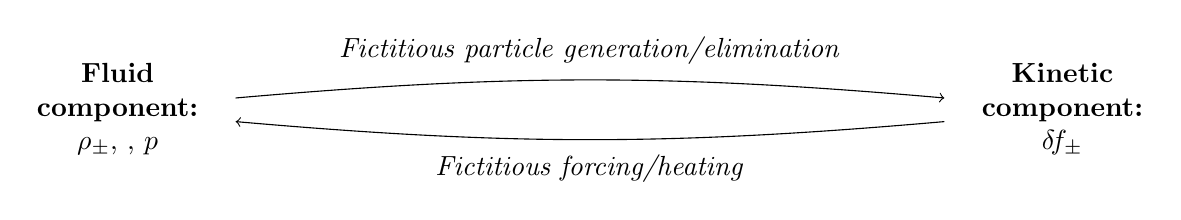
\begin{tikzpicture}[align = center, node distance = 4cm, auto]
            \node (1) at (0,  0) {\bf Fluid    \\  \bf component:  \\  $\rho_{\pm}$, $\bfp$, $p$};
            \node (2) at (12, 0) {\bf Kinetic  \\  \bf component:  \\  $\delta\! f_{\pm}$};
            
            \draw[->] (1.5, 0.15) to [out = 5, in = 175] (10.5, 0.15);
            \node at (6, 0.75) {\emph{Fictitious particle generation/elimination}};
            \draw[->] (10.5, - 0.15) to [out = 185, in = -5] (1.5, - 0.15);
            \node at (6, - 0.75) {\emph{Fictitious forcing/heating}};
        \end{tikzpicture}
        \caption{Illustration of the coupling between the fluid and kinetic components of a fully coupled $\delta\! f$ model.}
        \label{fig:delta f coupling}
    \end{figure}

    \BA{Need to include Maxwell's equations here too!}

    \BA{Check the coupled kinetic equation conserves moments.}
    